\documentclass[11pt]{article}
% Packages
\usepackage{times}
\usepackage[fleqn]{amsmath}
\usepackage{amssymb}
%\usepackage{anysize}
\usepackage{graphicx}
\usepackage{booktabs}
\usepackage{titlesec}
\usepackage{float}
\usepackage{natbib}
\usepackage[english]{babel}
\usepackage[autolanguage]{numprint}
\usepackage[tableposition=top]{caption}
\usepackage{subcaption}

% Macros
\newcommand{\np}{\numprint}
\newcommand{\tdl}{TD($\lambda$)}

% Options
%\marginsize{2.5cm}{1.5cm}{1cm}{1cm}

% Title spec
\title{%
  COMP3130 --- Group Project in Computer Science \\
  10$\times$10 Othello Learning Agent}
\date{June 8, 2012}
\author{%
  Andrew Haigh -- u4667010 \and
  Timothy Cosgrove -- u4843619 \and
  Joshua Nelson -- u4850020}

% Section styling
\titleformat{\section}%
  {\large\itshape}%
  {\thesection.}{.5em}{}%
  [\vspace{1ex}\titlerule]%
\titleformat{\subsection}%
  {\itshape}%
  {\thesubsection.}{.5em}{}%

% Document
\begin{document}
\maketitle
\begin{abstract}
An agent to play the board game \emph{Othello} is created, with the ability to
learn through reinforcement. The minimax algorithm is used for game playing,
and a static evaluation function for the leaf nodes is learnt by self play.
The agent learns the insignificance of the number of stones, and the
significance of stone positioning. This agent is played against itself, and
against other developed agents, and its performance is analysed.
\end{abstract}
\clearpage

\section{Problem overview}
%%Describe the game and the nature of the task

\section{Solution overview}
%%A minimax agent with a static evaluation function.

\section{Optimisations}
%% Alpha beta pruning, negamax, etc.

\section{Static evaluation function}
%% Necessity of a static evaluation function, features used, etc

\section{Learning}

\subsection{\tdl}

The \tdl\ algorithm was used to learn the weighting of the static evaluation
function's various features. The implementation of this algorithm is based on
the one implemented by the Knightcap agent as described by \citet{Baxter1997}.
At the end of each game played, the agent adjusts its weights according to
the following formula

\begin{center}

    $\displaystyle w := w + \alpha \sum _{t=1} ^{N-1} \Delta \tilde{J}(x_t,w) \: \times \: \Big[ \sum ^ {N-1} _{j=t} \lambda^{j-t} d_t \Big] $\\
        
    \begin{tabular}{  l l | l l }
      $w$                   & The vector of weights                         &$x_t$  & The $t^{th}$ board in the game \\
      $\alpha$              & The learning rate                             &$\lambda$      &The discount factor \\
      $N$                   & The number of states in the game              &$d_t$          &$\tilde{J}(x_{t+1},w) - \tilde{J}(x_t,w)$\\
      $\Delta \tilde{J}$    & The derivative of the $\tilde{J}$ function    &               &\\
    \end{tabular}
\end{center}

In the above formula, the $\tilde{J}$ function estimates the probability of
winning from a given state, given a set of weights for features and our board.
It approximates the $J$ function, \\

\begin{center}
$
J(x_t) = \begin{cases} 1, & \mbox{if } x_t\mbox{ is a winning state} \\ 0, & \mbox{if } x_t\mbox{ is a lost state} \end{cases}
$
\end{center}

For each game state $x_t$, we adjust the weights according to a factor $d_t$,
which is the temporal difference. $d_t = \tilde{J}(x_{t+1},w) -
\tilde{J}(x_t,w)$, and the weight adjustment is scaled with this amount. The
key observation is, for the true $J$ function, $J(x_{t+1}) - J(x_t) = 0$, so
we adjust our weights relative to this amount.

From Figure~\ref{fig:learned_j}, we can see that the
$\tilde{J}$ function, while not accurate for the entirety of the game, is able
to predict the results within the last 20 moves. In comparison,
Figure~\ref{fig:initial_j} indicates that the $\tilde{J}$ function
initially is a bad approximation, as even after losing a game, the estimated
probability of winning is high.

\begin{figure}[htbp]
  \begin{subfigure}{0.45\textwidth}
    \centering
    % TODO
    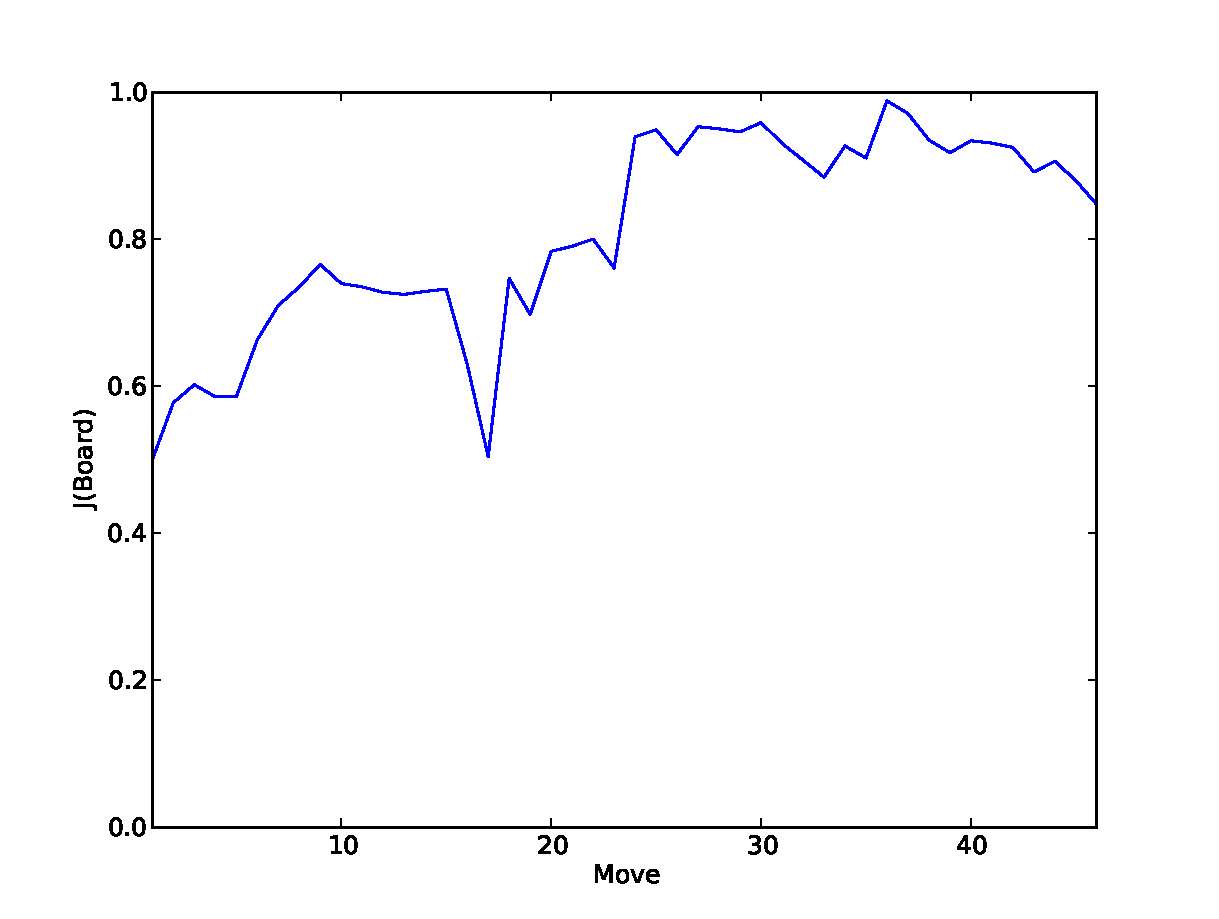
\includegraphics[width=\linewidth]{../Graphs/J_improved_1iteration_lost.pdf}
    \caption{Losing a game}
    \label{fig:initial_j_lost}
  \end{subfigure}
  \hspace{1em}
  \begin{subfigure}{0.45\textwidth}
    \centering
    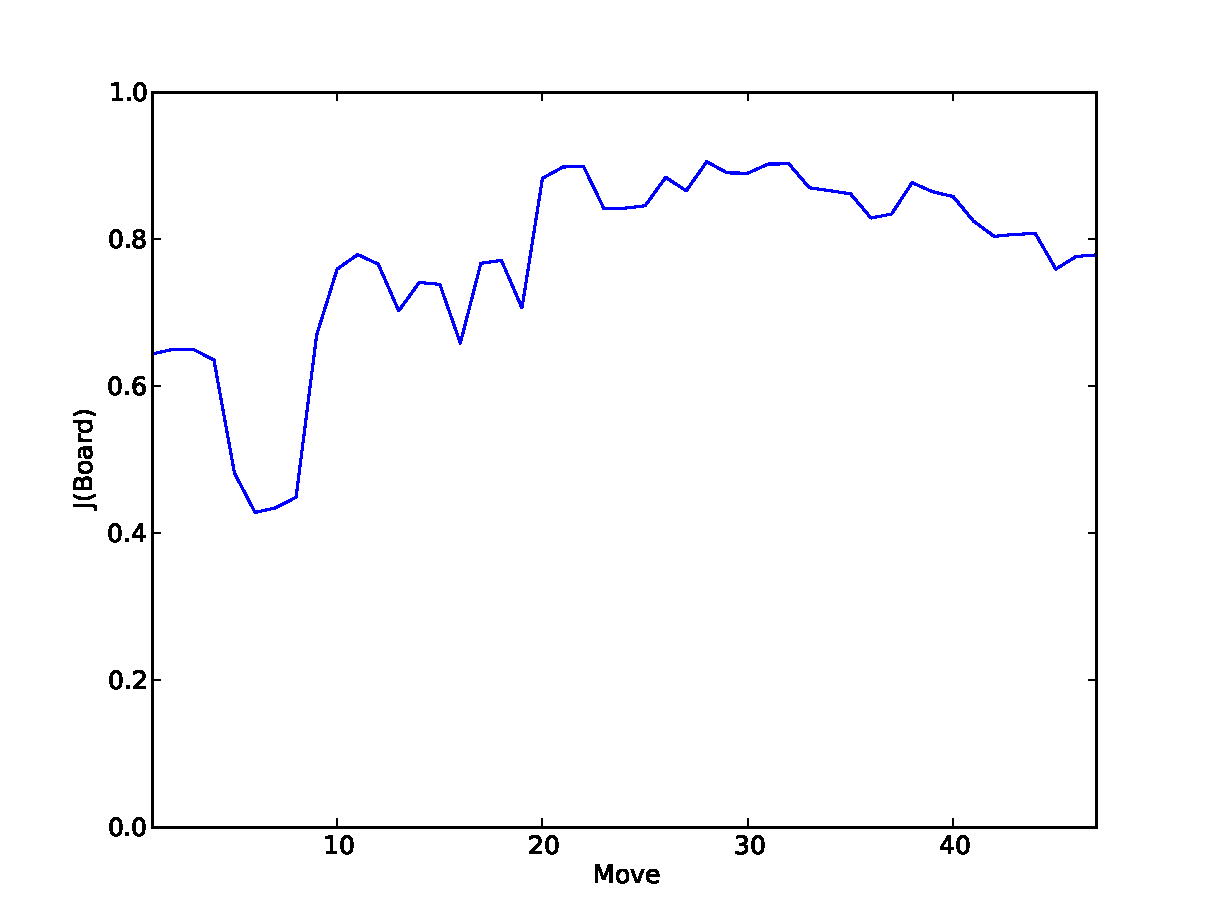
\includegraphics[width=\linewidth]{../Graphs/J_improved_1iteration_won.pdf}
    \caption{Winning a game}
    \label{fig:initial_j_win}
  \end{subfigure}
  \caption{$\tilde{J}$ Function initially}
  \label{fig:initial_j}
  %\label{JFunctionGraphs_1000iterations}
\end{figure}

\begin{figure}[htbp]
  \begin{subfigure}{0.45\textwidth}
    \centering
    % TODO
    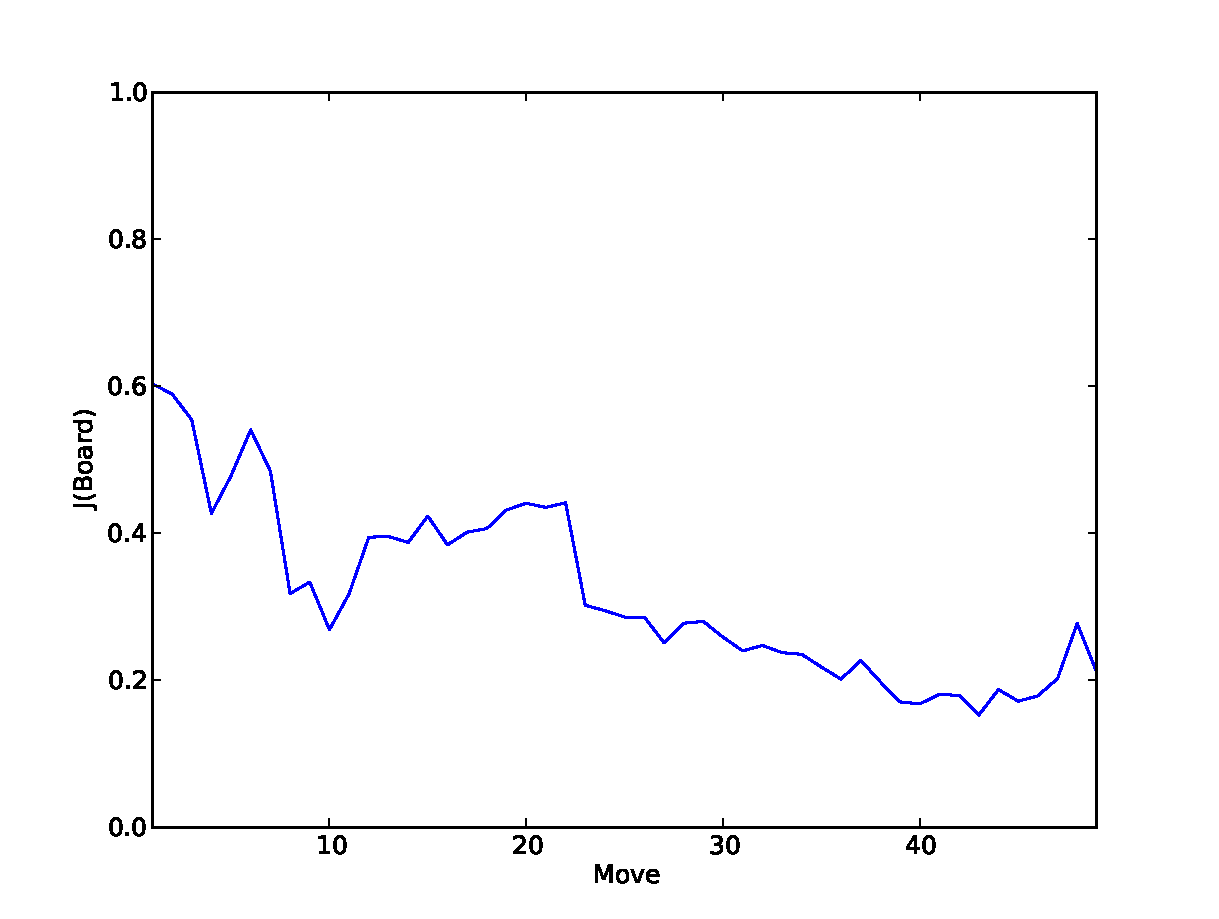
\includegraphics[width=\linewidth]{../Graphs/J_improved_1000iteration_lost.pdf}
    \caption{Losing a game}
    \label{fig:learned_j_lost}
  \end{subfigure}
  \hspace{1em}
  \begin{subfigure}{0.45\textwidth}
    \centering
    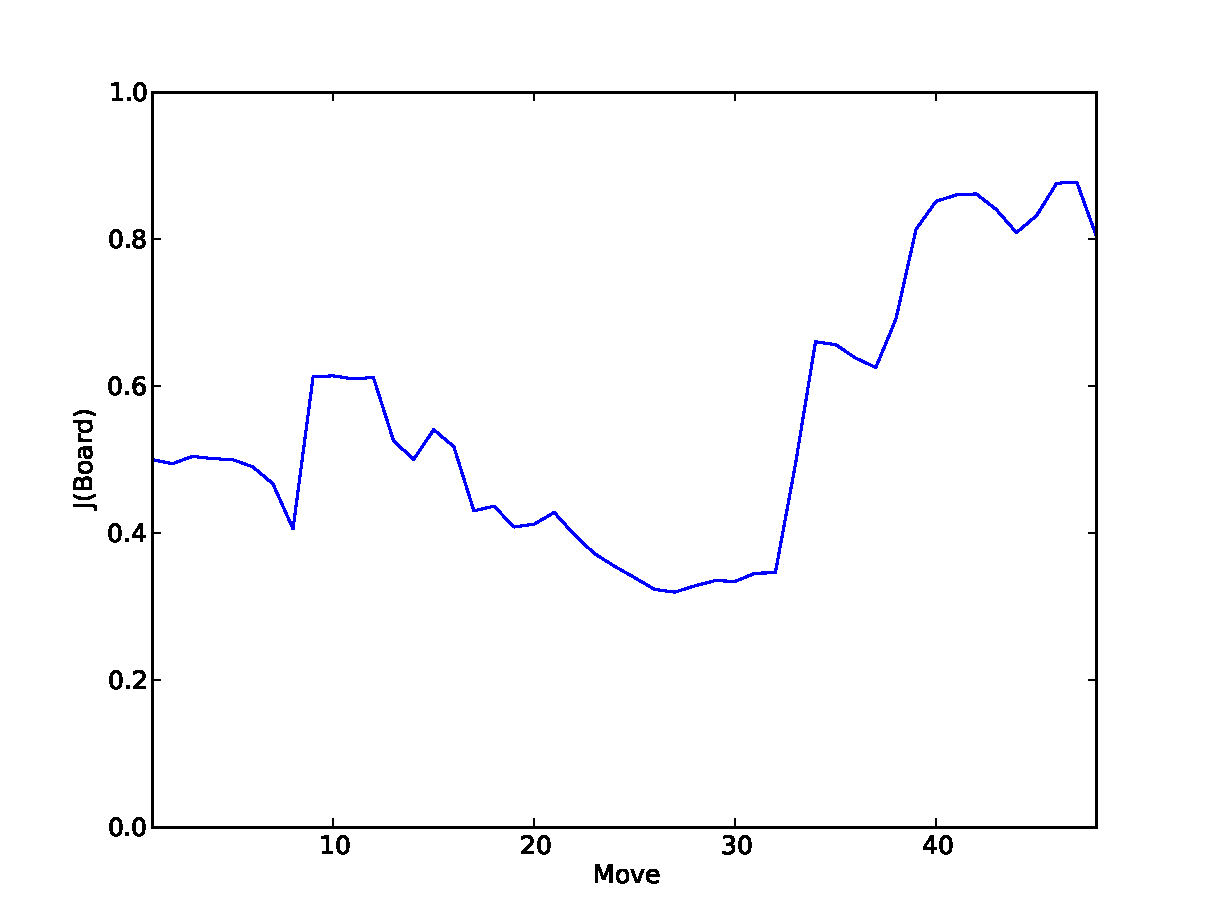
\includegraphics[width=\linewidth]{../Graphs/J_improved_1000iteration_won.pdf}
    \caption{Winning a game}
    \label{fig:learned_j_win}
  \end{subfigure}
  \caption{$\tilde{J}$ Function after 1000 learning iterations}
  \label{fig:learned_j}
  %\label{JFunctionGraphs_1000iterations}
\end{figure}

In Figure \ref{LearningProgress}, we can see the progress of the learning
agent as it plays against a fixed opponent. After about 1000 games, the agent
settles on a win/loss ratio of approximately 0.7.  The weights learnt were
split into 20 stages. Figure \ref{WeightsOverTime} shows the how highly the
various features are weighted as a game progresses. We see that the `Legal
Moves' feature is weighted highly early in the game, and later in the game,
valued less. On the other hand, corner pieces and side pieces become more
important as we approach the mid and end game. This makes sense, as the number
of legal moves on the board is limited later in the game, and it is unlikely
that a side or corner piece will be taken in the first quarter of the game.

\begin{figure}[htbp]
  % Currently the formatting of these graphs are terrible. I have no idea how
  % it can be fixed though unfortunately.
  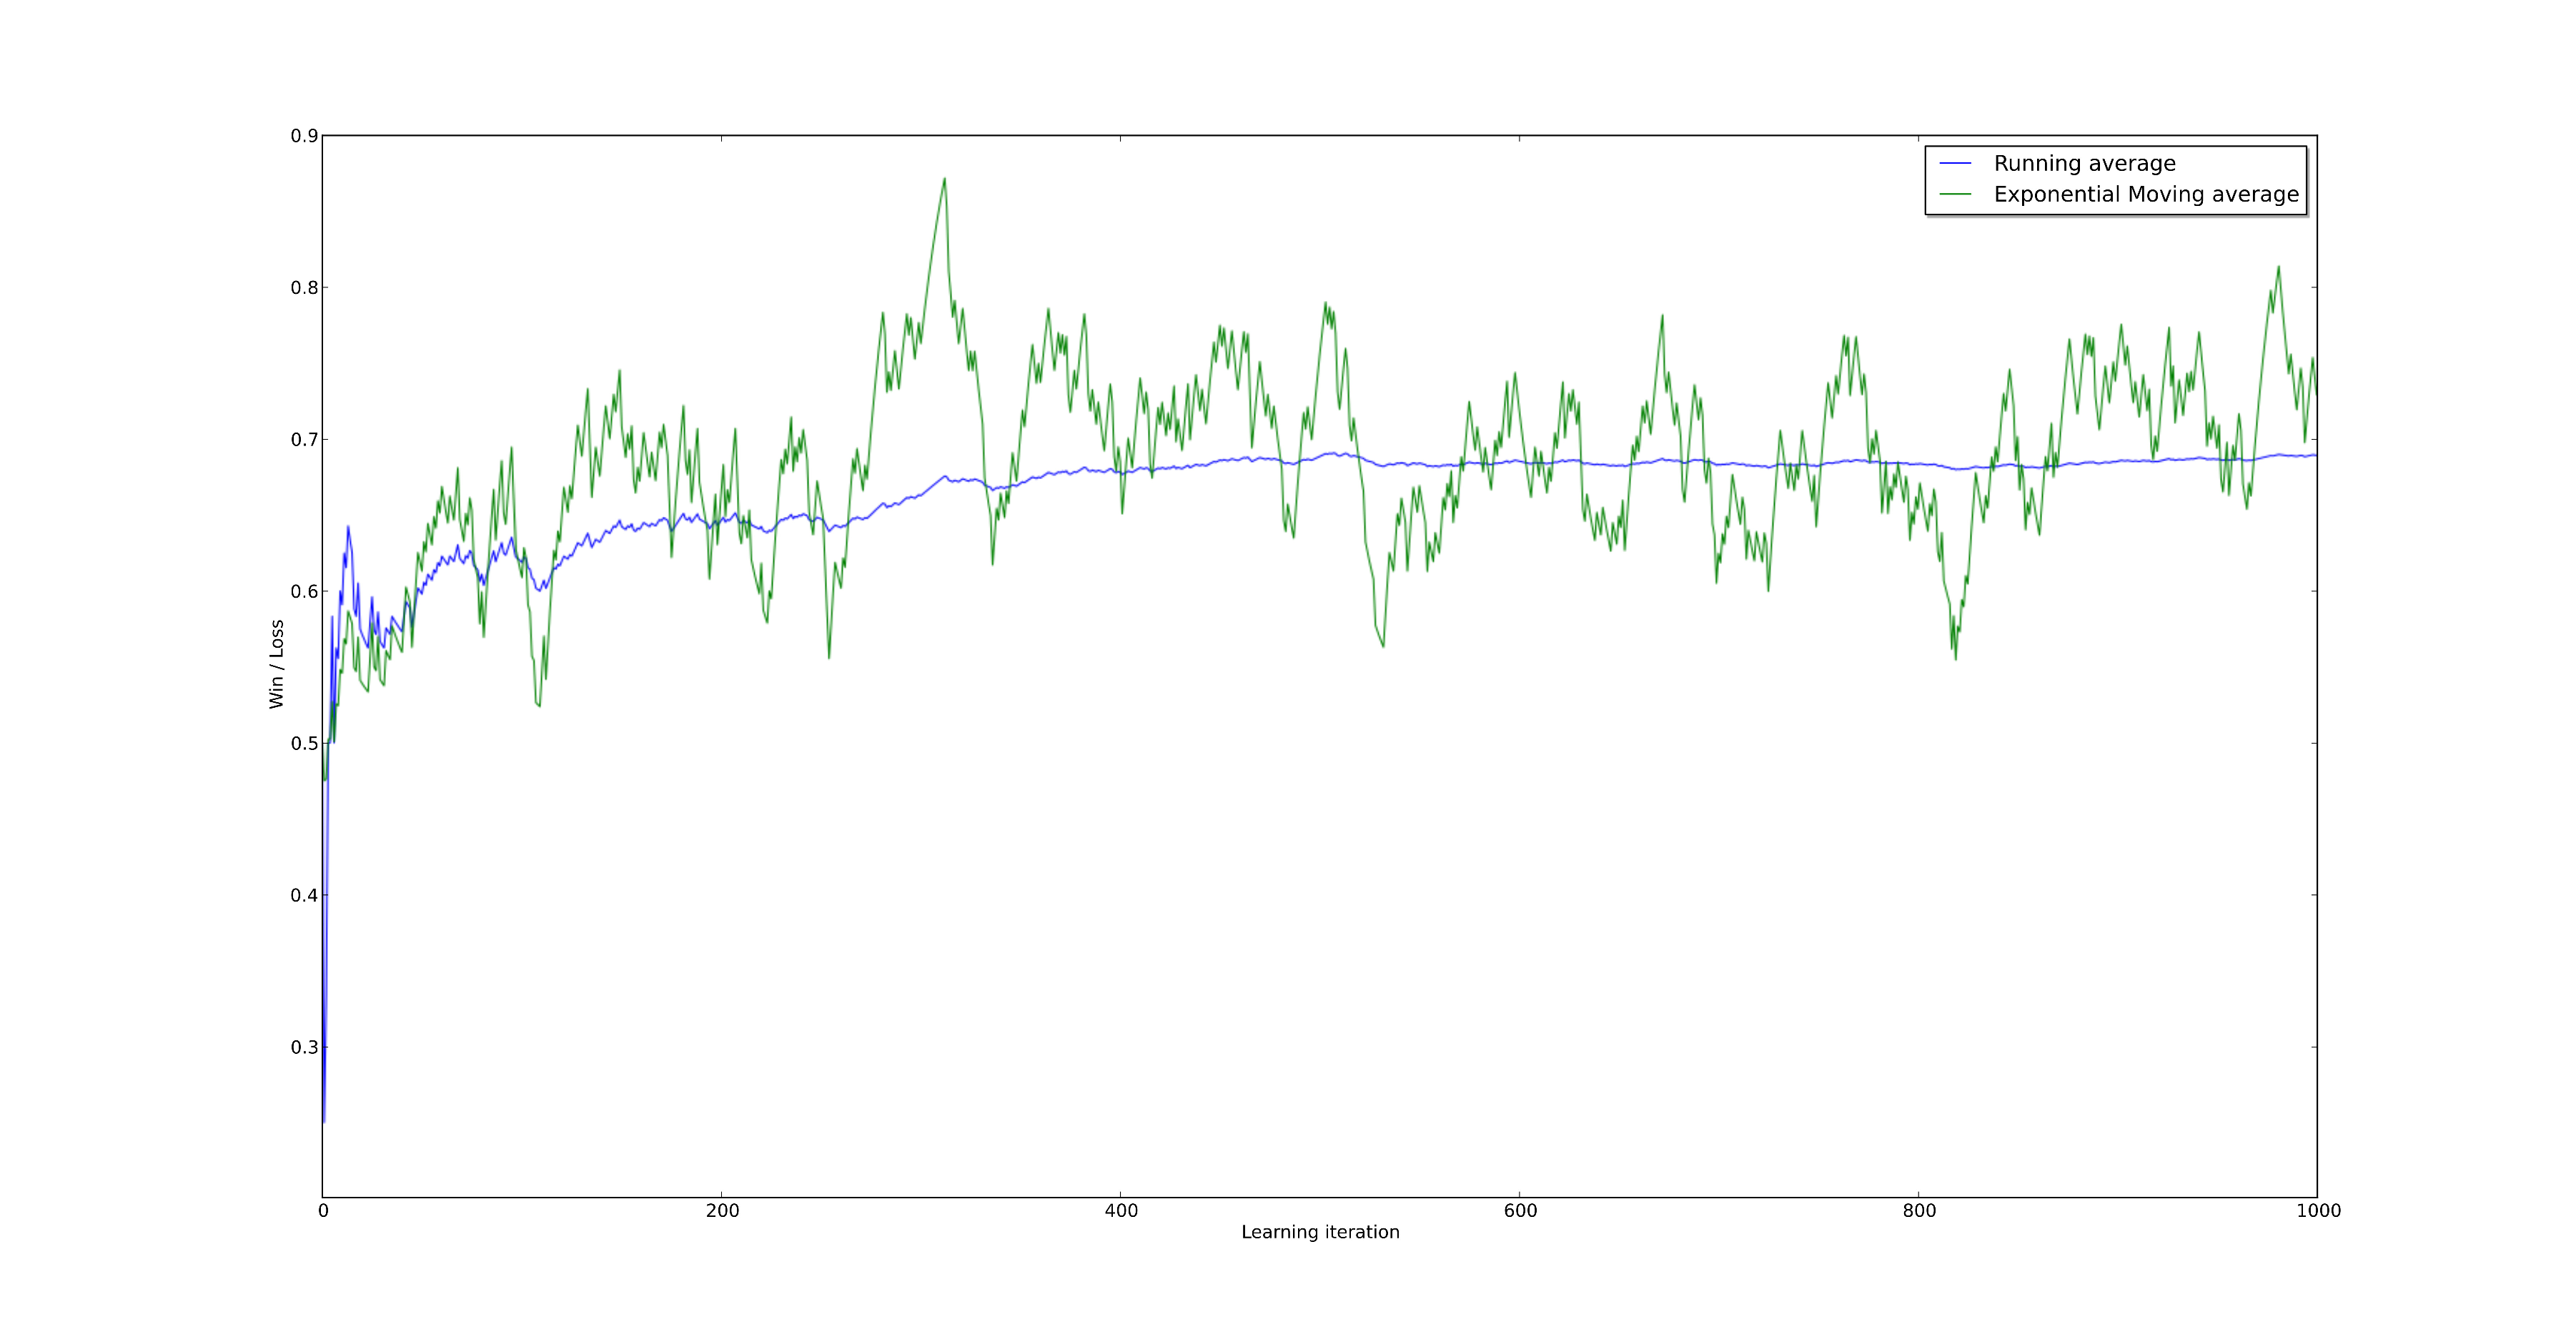
\includegraphics[width=1\textwidth]{../Graphs/Learning_2ply_First1000.pdf}
  \caption{Learning Progress of a 4-ply Learning player vs. a 4-ply Minimax
    player}
  \label{LearningProgress}
\end{figure}

\begin{figure}[htbp]
  \centering
  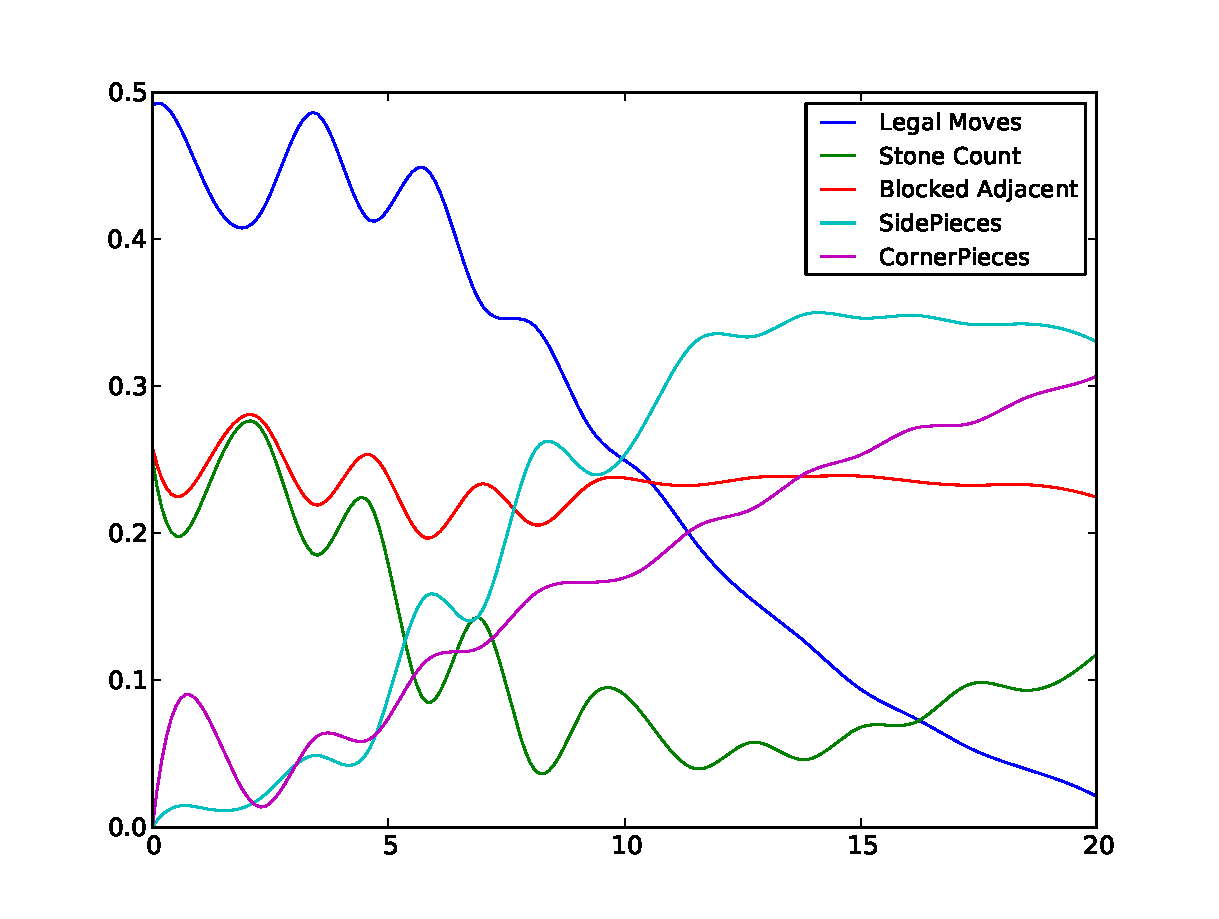
\includegraphics[width=0.75\textwidth]{../Graphs/WeightsOverTime.pdf}
  %%If you can come up with a better graph than this feel free to put it here
  \caption{Learned weights for a 20-stage player after 1000 learning
    iterations}
  \label{WeightsOverTime}
\end{figure}
%\clearpage

\subsection{ELO arena}

\subsection{Comparison of \tdl\ and ELO arena}
%% TD lambda and ELO arena

\section{Performance evaluation}
%% Tournament results, self play learning, fixed opponent results.

\section{Improvements}
%% Look at the performance and say what we could have improved.


\bibliographystyle{chicago}
\bibliography{ai}
\end{document}
